\documentclass[t]{beamer}
\usepackage{CJKutf8}
\usepackage{amsfonts}
    \usepackage{amsmath}
    \usepackage{amssymb}
    \usepackage{amsthm}
    \usepackage{enumerate}
    \usepackage{graphicx}
    \usepackage{layout}
    \usepackage{mathrsfs}
    \usepackage{fancyhdr}
    \usepackage{subfigure}
    \usepackage{tcolorbox}
    \usepackage{tikz-cd}
    \usepackage{color}
    \usepackage{pifont}
    \usepackage{verbatim}
    \usepackage{mathtools}
    \usepackage{float}
    \usepackage{bm}
    \usetheme{AnnArbor}
% \usetheme{Antibes}
\usecolortheme{beaver}
\usepackage{listings}

% 设置JSON样式
\lstdefinestyle{json}{
    basicstyle=\tiny\ttfamily,
    columns=fullflexible,
    showstringspaces=false,
    commentstyle=\color{gray},
    keywordstyle=\color{blue},
    stringstyle=\color{red},
    breaklines=true,
    frame=single,
    captionpos=b,
    aboveskip=10pt,
    belowskip=10pt
}

\lstset{
    language=Python, % 设置代码块语言为Python
    breaklines=true, % 自动换行
    basicstyle=\small\ttfamily, % 设置基本字体样式
    keywordstyle=\bfseries\color{blue}, % 设置关键字样式
    commentstyle=\itshape\color{gray}, % 设置注释样式
    showstringspaces=false, % 不显示字符串中的空格
    frame=single, % 设置代码块边框样式
    numbers=left, % 行号显示在左侧
    numberstyle=\tiny\color{gray}, % 设置行号样式
    stepnumber=1, % 设置行号间隔
    tabsize=4 % 设置制表符宽度
}


% 设置shell样式
\lstdefinestyle{shell}{
    language=bash,
    basicstyle=\tiny\ttfamily,
    columns=fullflexible,
    showstringspaces=false,
    commentstyle=\color{gray},
    keywordstyle=\color{blue},
    stringstyle=\color{red},
    breaklines=true,
    frame=single,
    captionpos=b,
    aboveskip=10pt,
    belowskip=10pt
}

% 添加网址的命令
\usepackage{hyperref}
% 这是一个带链接文本的示例:\href{https://www.example.com}{点击这里访问网站}
% 普通的示例:\url{https://www.example.com}
% 表格
\usepackage{booktabs}
\usepackage{multirow}

% \setbeamertemplate{navigation symbols}{}

\usepackage{textpos}

\newcommand{\dif}{\mathrm{d}}
\newtheorem{thm}{{定理}}

% some common command
\newcommand{\mm}[1]{$ #1$\newline}
% \newcommand{\tuichu}{\Rightarrow}
% \newcommand{\li}[1]{\newline#1}



\newcommand{\analysis}[2]{\forall \mathcal{E}{#1},\exists \delta {#2},s.t.}
\newcommand{\denyanalysis}[2]{\exists \mathcal{E}{#1},\forall \delta {#2},s.t.}
\newcommand{\yield}{\Rightarrow }
\newcommand{\jj}{\newline}
\newcommand{\ff}[1]{$ #1$}   % math environment + newline
\newcommand{\fgn}[1]{\begin{equation}#1\end{equation}  }
\newcommand{\fg}[1]{$$ #1$$}   % math environment + newline 
\newcommand{\pf}{$proof.$\newline}
\newcommand{\ee}{\newline\ff{\Box}\newline}
\newcommand{\fenshi}[2]{\ff{\frac{#1}{#2}}}
\newcommand{\shenlue}{\vdots\jj}
\newcommand{\abs}[1]{{\left \lvert #1 \right\rvert}}
\newcommand{\loge}[1]{In ({#1})}
\newcommand{\logical}[2]{log_{#2}^{#1}}
\newcommand{\summary}[3]{$\sum_{{#1}={#2}}^{#3}  $}
\newcommand{\denjia}[2]{{#1}\Leftrightarrow {#2}}
\newcommand{\jihe}[3]{ {#1}  = \{ {#2} \mid {#3} \} }
\newcommand{\ve}[2]{\left\langle {#1},{#2}\right \rangle}
\newcommand{\dakuohao}[2]{\begin{array}{rcl}{#1}\end{array} \} \Rightarrow{#2}}
\newcommand{\sxb}[3]{#1^{#2}_{#3}}
\newcommand{\sss}[2]{#1^{#2}}
\newcommand{\xxx}[2]{#1_{#2}}
\newcommand{\bri}[1]{\uppercase\expandafter{\romannumeral#1}}
\newcommand{\ri}[1]{\romannumeral#1} 
\newcommand{\polynomial}[8]{#1_{#2}#6^{#7}+#1_{#3}#6^{#8}+...+#1_{#4}#6+#1_{#5} }
\newcommand{\newd}[4]{f[{#1}_{#2},{#4},{#1}_{#3}]}
\newcommand{\lb}[2]{\begin{align*}\begin{split}{#1}\{ {#2}\end{split}\end{align*}}
\newcommand{\tab}[1]{\begin{array}{ll} {#1}\end{array}}


% 向量乘积
\newcommand{\avg}[1]{\left\langle #1 \right\rangle}
% 偏微分方程
\newcommand{\difFrac}[2]{\frac{\dif #1}{\dif #2}}
\newcommand{\pdfrac}[2]{\frac{\partial{#1}}{\partial{#2}}}
% 不同章节
\newcommand{\one}[1]{\section{#1}}
\newcommand{\two}[1]{\subsection{#1}}
\newcommand{\three}[1]{\subsubsection{#1}}
\newcommand{\aone}[1]{\section*{#1}}
\newcommand{\atwo}[1]{\subsection*{#1}}
\newcommand{\athree}[1]{\subsubsection*{#1}}
% 大括号,左右都有
\newcommand{\lbra}[1]{\left\{  {\begin{matrix} #1 \end{matrix}}\right. } 
% 样式 括号前缀 + 括号 
\newcommand{\lbras}[2]{{#1}\left\{ {  {\begin{matrix} #2 \end{matrix}}}\right. } 
\newcommand{\rbra}[1]{ \left.  {\begin{matrix} #1 \end{matrix}} \right\}  } 
% 模长
\newcommand{\distance}[1]{\parallel #1\parallel }
% 等价
\newcommand{\equ}{\Longleftrightarrow }
% 共轭
\newcommand{\cja}[1]{\overline{#1}}
% 两个矩阵,上面是 方框[] 下面是线条| 中间是 无
\newcommand{\mtx}[1]{\begin{matrix}#1\end{matrix} }
\newcommand{\bmtx}[1]{\begin{bmatrix}#1\end{bmatrix} }
\newcommand{\vmtx}[1]{\begin{vmatrix}#1\end{vmatrix} }
% \newcommand{\table}[1]{\begin{array}[lr]{ccc} #1 \end{array}}

%输入普通字符
\newcommand{\ww}[1]{\text{#1}}

% 所有内容 直接头文件搞定
\newcommand{\everything}[1]{\begin{document}\begin{CJK*}{UTF8}{gkai}#1\end{CJK*}\end{document}}


% 存放代码(失败了)
\newcommand{\cccode}[1]{\begin{lstlisting}#1\end{lstlisting}}

% 改变特定行序列
\newcommand{\ttt}{\subsection{}}

% 嵌套序号
\newcommand{\eee}[1]{\begin{enumerate}#1\end{enumerate}}


% 模板里面的一些宏
\newcommand{\pdfFrac}[2]{\frac{\partial #1}{\partial #2}}
\newcommand{\OFL}{\mathrm{OFL}}
\newcommand{\UFL}{\mathrm{UFL}}
\newcommand{\fl}{\mathrm{fl}}
\newcommand{\op}{\odot}
\newcommand{\Eabs}{E_{\mathrm{abs}}}
\newcommand{\Erel}{E_{\mathrm{rel}}}
% 变化颜色
\newcommand{\red}{\textcolor{red}}
\newcommand{\blue}{\textcolor{blue}}
% 注释代码
% \newcommand{\undef}[1]{\iffalse #1 \fi}

% 流程图需要用到的宏包
\usepackage{palatino}
\usepackage{tikz}
\usetikzlibrary{shapes.geometric, arrows}
\tikzstyle{startstop} = [rectangle, rounded corners, minimum width = 2cm, minimum height=1cm,text centered, draw = black, fill = red!40]
\tikzstyle{io} = [trapezium, trapezium left angle=70, trapezium right angle=110, minimum width=2cm, minimum height=1cm, text centered, draw=black, fill = blue!40]
\tikzstyle{process} = [rectangle, minimum width=3cm, minimum height=1cm, text centered, draw=black, fill = yellow!50]
\tikzstyle{decision} = [diamond, aspect = 3, text centered, draw=black, fill = green!30]
% 箭头形式
\tikzstyle{arrow} = [->,>=stealth]
% 4个非常重要 的新命令
\newcommand{\start}[2]{    \node (start) [startstop]{#1};\node (in1) [io, below of = start]{#2};\lin{start}{in1}{}}
\newcommand{\stopp}[3]{\node (out1) [io, below of= #1]{#2};\node (stop) [startstop, below of=out1]{#3};\lin{out1}{stop}{} }
\newcommand{\pro}[6]{    \node (#3) [process, #2 of=#1,xshift=#4 cm]{#5};}
\newpage
\newcommand{\lin}[3]{\draw [arrow] (#1) --node [above] {#3} (#2);}


\begin{document}
\begin{CJK*}{UTF8}{gkai}
% 一般第一页显示PPT标题以及作者信息

% \BackgroundPic{./Screenshot from 2022-04-20 16-31-08.png}

% 增加学校 前面
\addtobeamertemplate{title page}{}{
	\begin{tikzpicture}[remember picture,overlay]
		% \node[yshift=85pt,xshift=50pt]{\includegraphics[height=2cm]{Screenshot from 2022-04-20 16-51-21.png}};
\end{tikzpicture}
}


	% \title{时间序列数据集}
	\title{组会汇报}
	\subtitle {} %不需要
	\author{
		陈钶杰\, \\
		专业:计算数学\,
	} % 显示作者
	% \institute {学院:数学科学学院} % 设置学院机构	
	\date{\today}  % 显示日期
\titlepage

% 设置目录
\begin{frame}{目录}
\frametitle{目录}	
\tableofcontents  % 显示目录
\end{frame}


\section{相关的论文}

% \begin{frame}
%     \frametitle{论文:少量学习的神经机制}
%     \begin{itemize}
%         % \item 该论文提出了一种对自然主义概念进行少量学习的神经机制,这种机制在生物学上是合理的,在数学上是可处理的,而且计算能力强大。作者开发了一种关于少量学习的数学理论,该理论通过描绘神经表现的几个基本且可测量的几何特性,将神经生理学与行为结果的预测联系起来,这些特性可以准确预测自然主义概念的少量学习表现。
%         % \item 论文的导言突显了人类仅从一种或几种感官体验中学习新概念的非凡认知能力,这构成了一个基本问题。作者提出了一种简单、生物学上合理、数学上可处理且计算能力强大的神经机制,用于对自然主义概念的几次学习。他们认为,可以从几个例子中学到的概念是由高阶感官区域的神经射速空间中严格限制的流形来定义的。作者还讨论了理解神经回路在高维和低维神经表示之间进行权衡的理论原理的重要性。
%         % \item 该论文展示了拟议的少拍学习神经机制的计算能力,证明了它可以使用猕猴颞下皮层表示和这些表示的深度神经网络(DNN)模型在自然视觉概念上实现很高的少拍学习精度。作者还开发了一种关于少量学习的数学理论,该理论通过描绘神经表现的几个基本且可测量的几何特性,将神经生理学与行为结果的预测联系起来,这些特性可以准确预测自然主义概念在所有数值模拟中的少量学习表现。该理论表明,高维流形增强了从几个例子中学习新概念的能力。作者还讨论了他们的心理物理学和神经生理学实验理论的可检验预测。
%         \item 这篇文章是\red{关于了解人类如何从一个或几个感官经验中学习新概念的神经基础是神经学科一个基本问题}。作者提出了一个简单的、生物学上合理、数学上可操作、计算上强大的神经机制,用于对自然概念的小样本学习。作者认为,\red{可以从少数例子中学习}的概念是由高阶感觉区的神经放电率空间中严格限定的流形所定义的。作者进一步假设,一个单一的可塑性下游读出神经元通过一个简单的可塑性规则学会根据少数例子来辨别新概念。作者展示了此想法的计算能力,表明它可以使用猕猴下颞叶皮层表征和这些表征的深度神经网络模型在自然视觉概念上达到很高的学习精度,甚至可以学习仅通过语言描述符指定的新视觉概念。此外,作者开发了一个关于小样本学习的数学理论,通过描述神经表征的几个基本和可测量的几何特性,将神经生理学与行为结果的预测联系起来,这些特性可以准确地预测所有数字模拟的自然概念的小样本学习表现。这一理论显示,\red{高维流形增强了从少数例子中学习新概念的能力。}
%     \end{itemize}
% \end{frame}

\begin{frame}
    \frametitle{论文:Auto-CoT}
    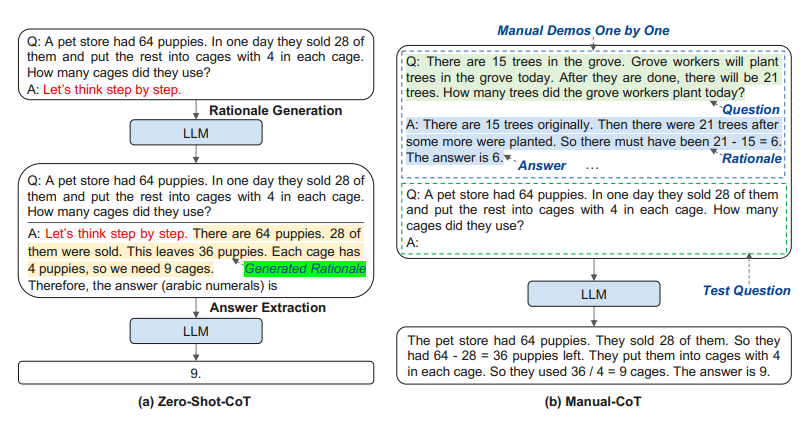
\includegraphics[scale=0.3]{png/auto_cot.png}
    \begin{itemize}
        \item 背景:复杂的问题需要中间步骤来解决,这个中间步骤就需要用到我们的思维链的方法。
        % 核心思路图片
        % \item 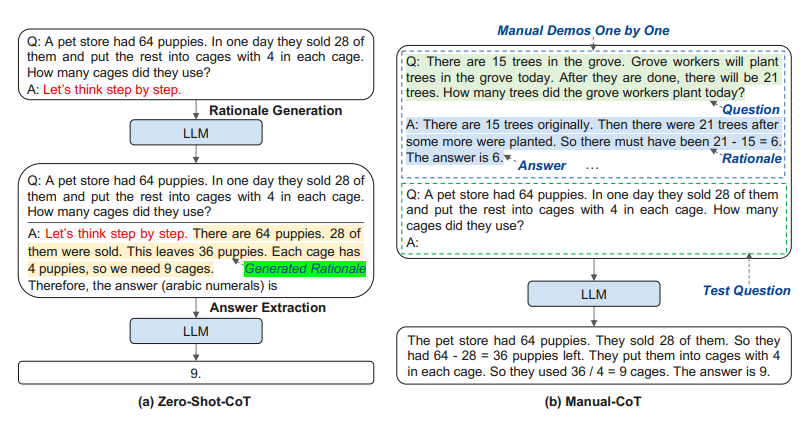
\includegraphics[scale=0.5]{png/auto_cot.png}
        % \item Auto-CoT这种方法的想法就是先从zero-shot里面将这个推导加入一个"let's think step by step"来引出answer,然后将这个问题和回答当作是few-shot里面的样例,如此就做到了让模型自动进行思维链回答。
        \item Auto-CoT这种方法的想法就是自动产生Manual-CoT中的微调数据集。在问题后加入一个"let's think step by step"来推导出answer,然后将这个问题和回答当作微调数据集。
    \end{itemize}
\end{frame}

\begin{frame}
    \frametitle{论文:Auto-CoT}
    \begin{itemize}
        \item 如何选择的问题数据集?\\
        \eee{
            \item 检索式:检索特定的问题集:\\
            % 问题原因:zero-shot可能产生错误的推理,导致最终效果不好了\\
            \item 随机式:随机寻找k个问题\\
            % 问题原因:选择更加有多样性,所以效果更好!
            \item 使用聚类的方法,将n个问题通过聚类分成k个集群,然后在每个集群里面找出最优的s个问题,组成的问题集来进行zero-shot learning得到我们想要的微调数据。
        }
        \item 结论:通过实验发现,在处理一些复杂问题时,使用Auto-CoT方法得到的结果准确性接近于Manual-CoT方法,明显优于Zero-Shot-CoT方法。
    \end{itemize}
\end{frame}

% \begin{frame}
%         \frametitle{一些知识}
%         \begin{itemize}
%             % \item LeCun坚持认为“大型语言模型本身永远无法实现真正的理解,"即使从现在起一直训练到宇宙热死"。
%             \item 
%         \end{itemize}
% \end{frame}

\section{langchain}
\begin{frame}
    \frametitle{langchain}
    \begin{itemize}
        \item LangChain是一个开源框架,允许从事人工智能的开发者将例如GPT-4的大语言模型与外部计算和数据来源结合起来。
        % \item LangChain是一种让将语言模型封装的工具,通过使用LangChain可以更加方便的使用语言模型的一些功能。
        % \item 能否将本地的glm与langchain部署起来。然后挖掘langchain的新功能吧,就这样吧,这周我就介绍一下什么是langchain。
        \item LangChain自身并不开发LLMs,它的核心理念是为各种LLMs实现通用的接口,把LLMs相关的组件“链接”在一起,简化LLMs应用的开发难度,方便开发者快速地开发复杂的LLMs应用。
        \item LangChain这是一个通用的框架,之后可以考虑用LangChain作为接口来做一些复杂的测试。
        % 如复杂的运算。
    \end{itemize}
\end{frame}

\begin{frame}
    \frametitle{主要技术路线}
    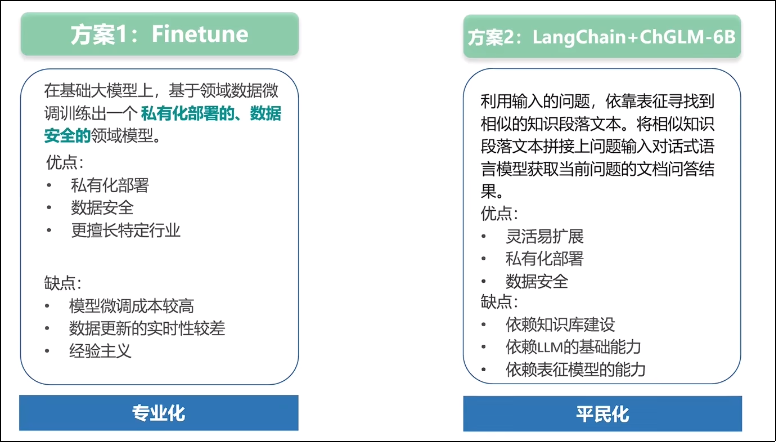
\includegraphics[scale=0.4]{png/langchain-chatglm.png}
\end{frame}

\begin{frame}
    \frametitle{具体使用的例子}
    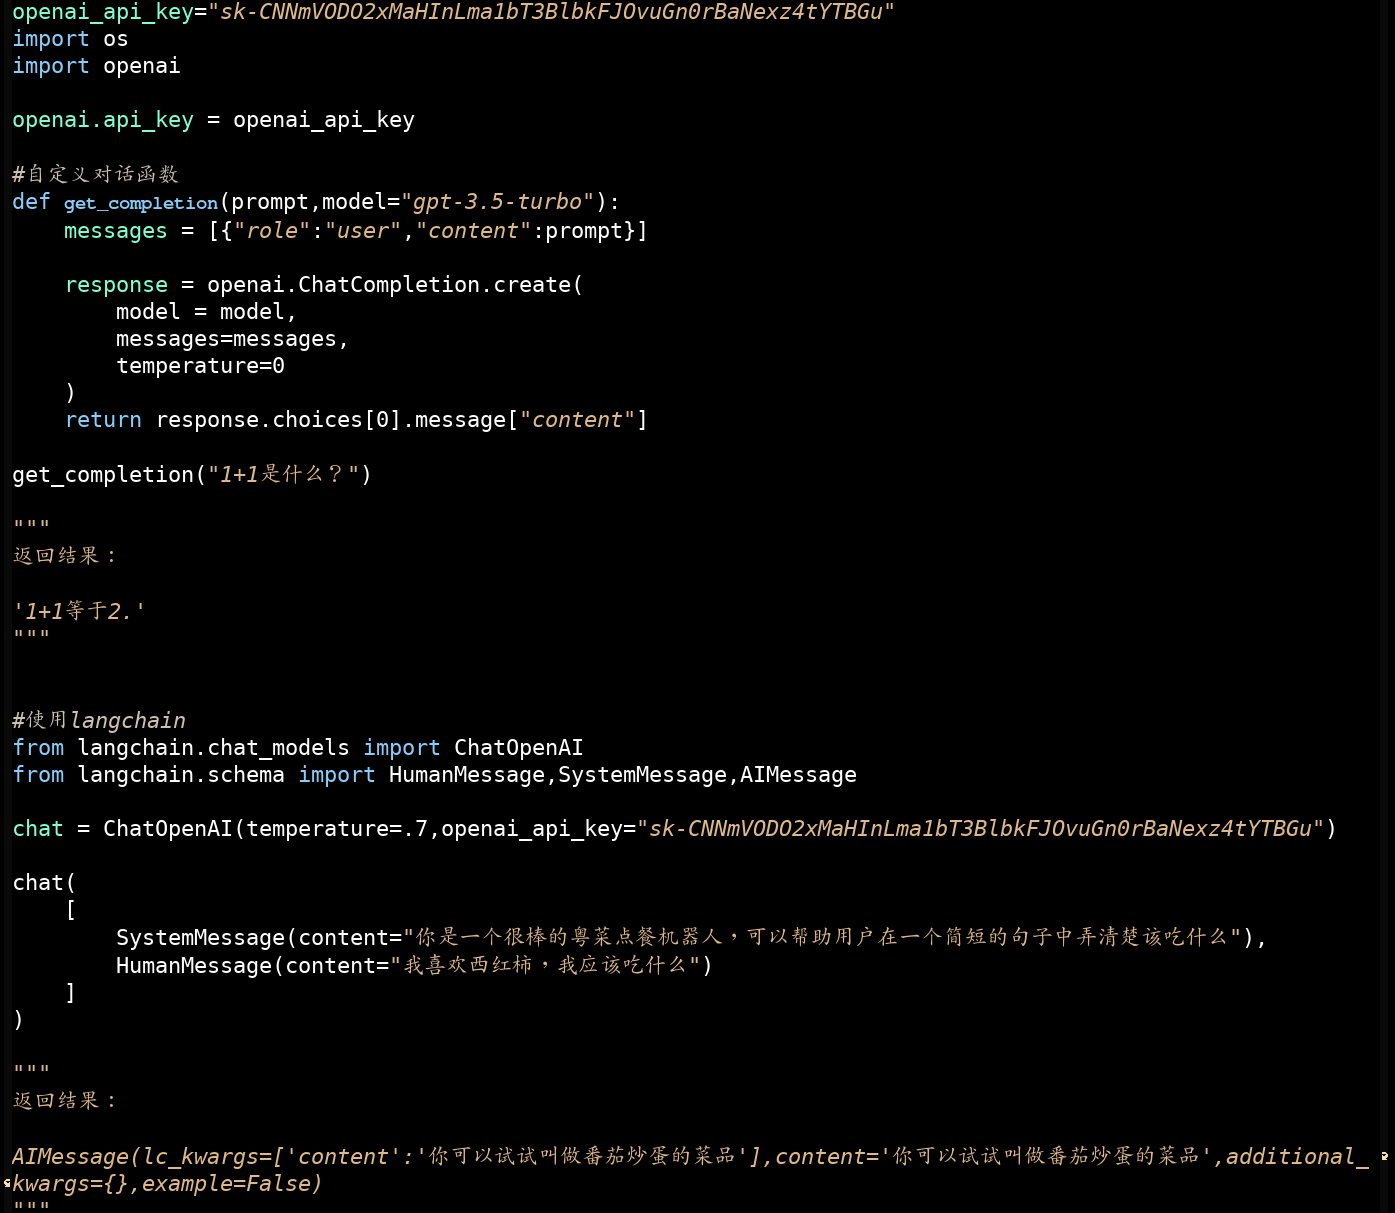
\includegraphics[scale=0.175]{png/langchain.png}
    % \begin{itemize}
    %     \item 如何使用llama
    %     \item 
    % \end{itemize}
\end{frame}

\section{代码调试相关}

\subsection{使用粗粒化,逐步推导的方式进行多步预测序列}

\begin{frame}
    \frametitle{\small (数据样例1)在见过的任务中粗粒化的测试结果,通过率是100\%}
	\begin{itemize}
        \item 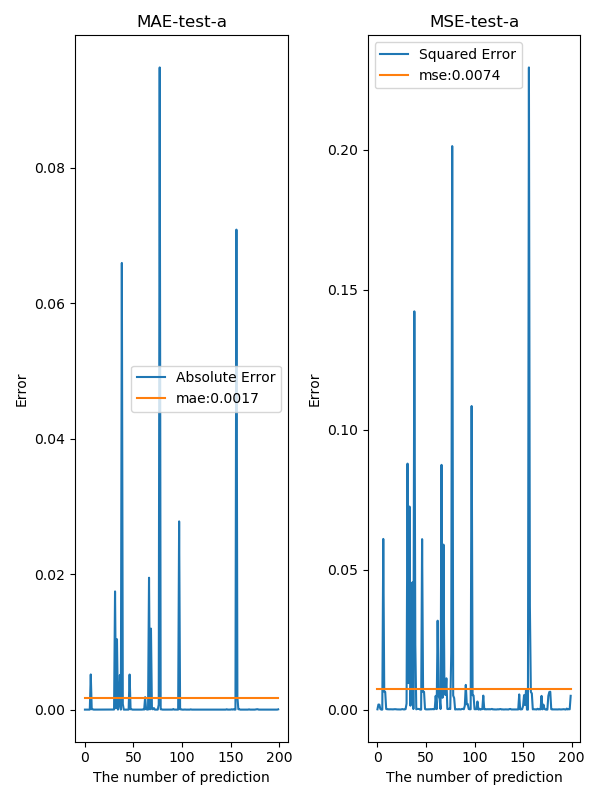
\includegraphics[scale=0.3]{png/test-a.png}		
	\end{itemize}
\end{frame}

\begin{frame}
    \frametitle{\small (数据样例1)在见过的任务上未进行粗粒化的测试结果}
	\begin{itemize}
        \item 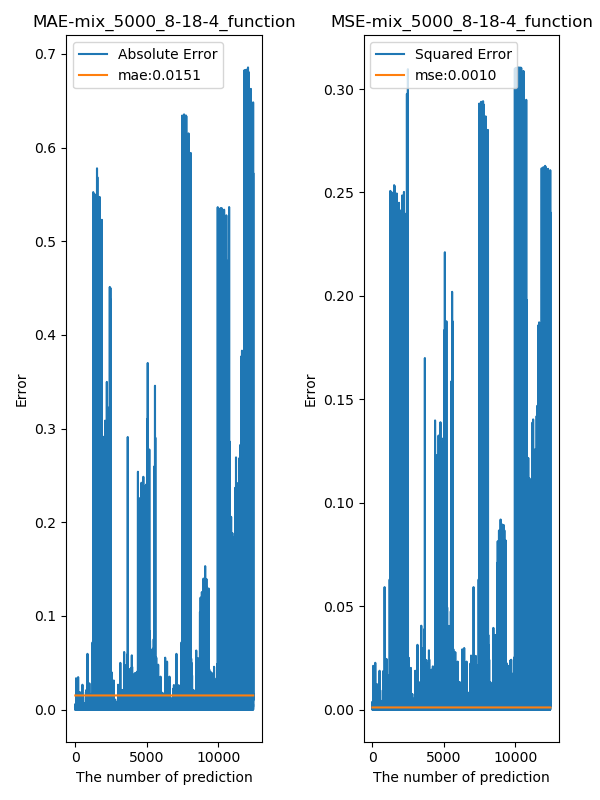
\includegraphics[scale=0.3]{png/mix_5000_8-18-4_function.png}
	\end{itemize}
\end{frame}

\begin{frame}
    \frametitle{\small (数据样例1)在没见过的任务上使用粗粒化的测试结果,通过率是88.5\%}
	\begin{itemize}
        \item 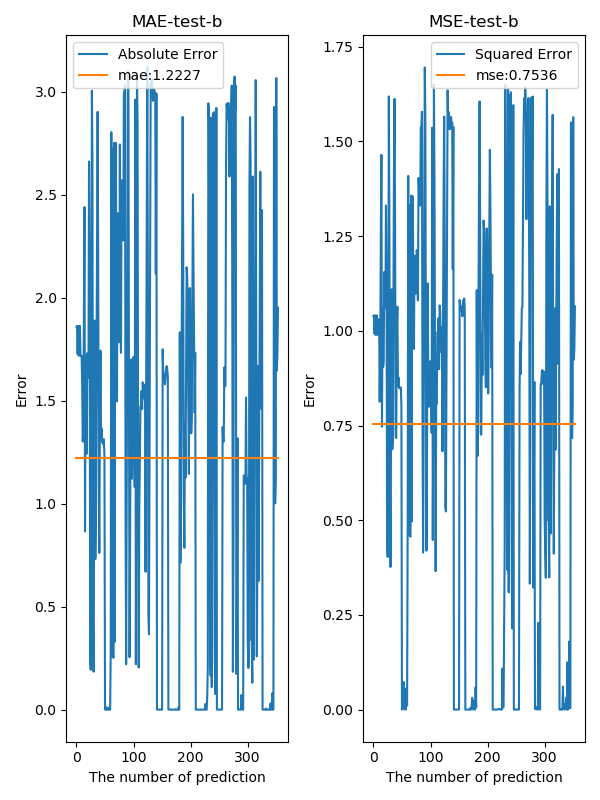
\includegraphics[scale=0.3]{png/test-b.png}
	\end{itemize}
\end{frame}


\begin{frame}
    \frametitle{\small (数据样例2)在见过的任务上使用逐步推导的测试结果,通过率是73.53\%}
	\begin{itemize}
        \item 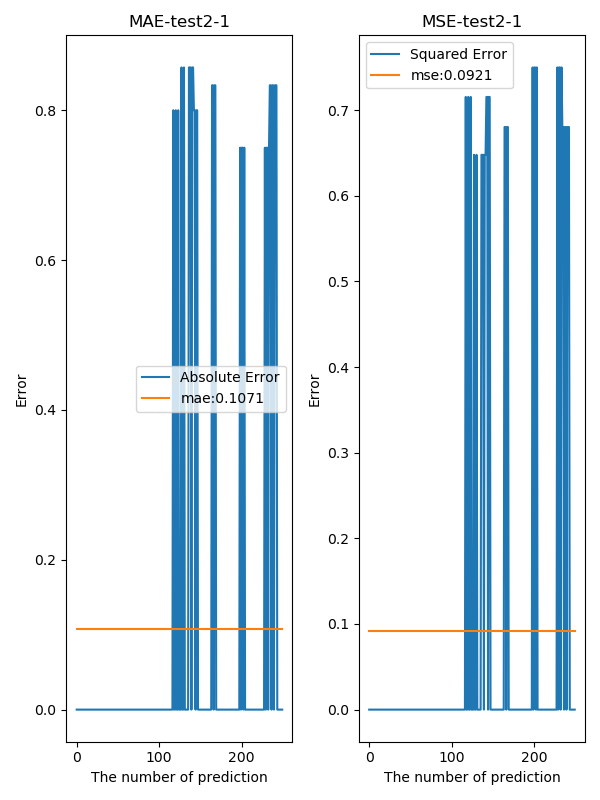
\includegraphics[scale=0.3]{png/test2-1.png}
	\end{itemize}
\end{frame}

\begin{frame}
    \frametitle{\small (数据样例2)在未见过的任务上使用逐步推导的测试结果,通过率是50.54\%}
	\begin{itemize}
        \item 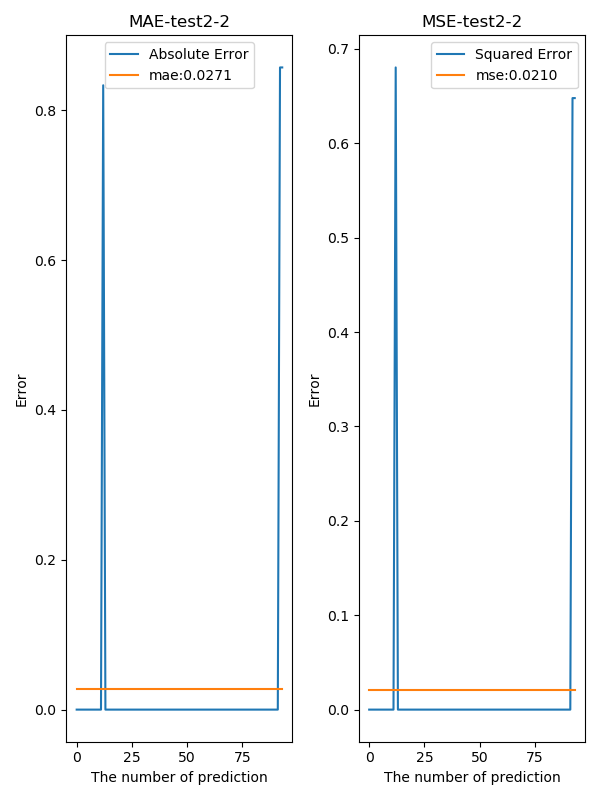
\includegraphics[scale=0.3]{png/test2-2.png}
	\end{itemize}
\end{frame}

\begin{frame}
    \frametitle{\small (数据样例2)在见过的任务上使用粗粒化的测试结果,通过率是97.5\%}
	\begin{itemize}
        \item 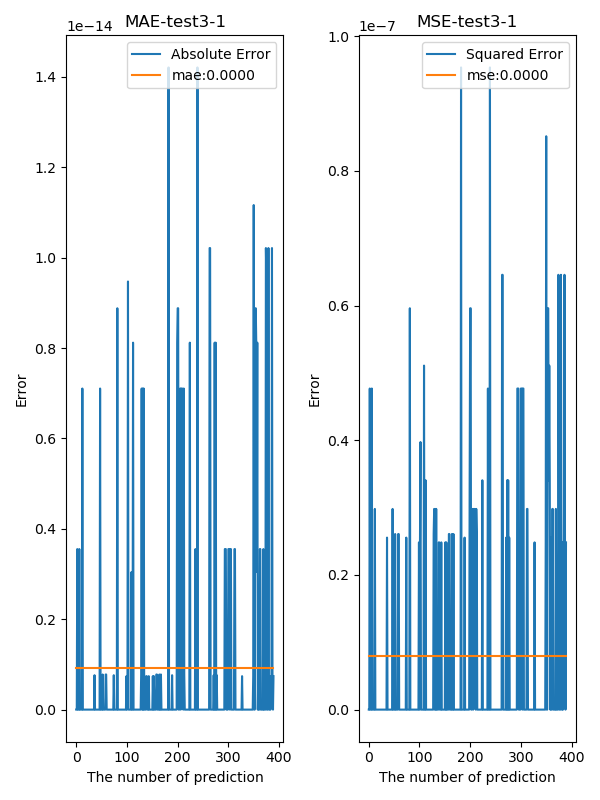
\includegraphics[scale=0.3]{png/test3-1.png}
        % \item MAE: tensor(9.3009e-16)\\
        % MSE: tensor(7.9418e-09)
	\end{itemize}
\end{frame}

\begin{frame}
    \frametitle{\small (数据样例2)在未见过的任务上使用粗粒化的测试结果,通过率是75.5\%}
	\begin{itemize}
        \item 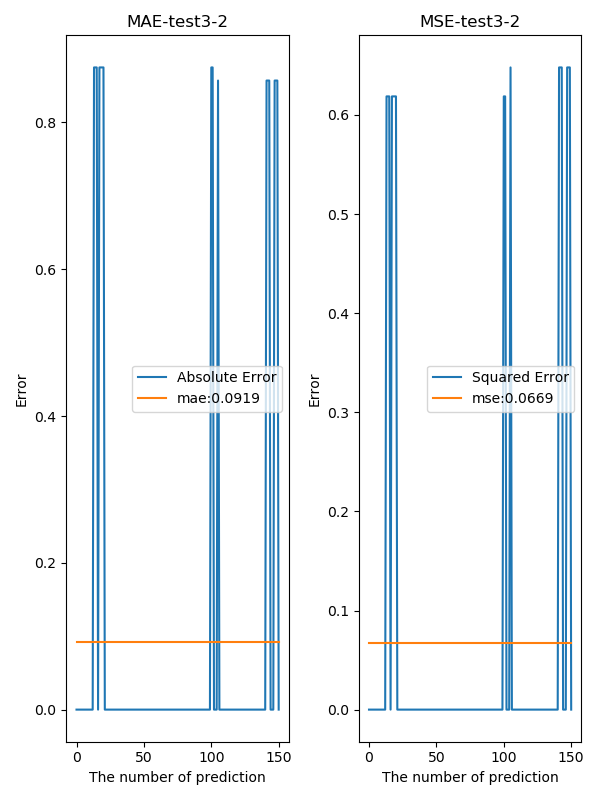
\includegraphics[scale=0.3]{png/test3-2.png}
	\end{itemize}
\end{frame}


\subsection{给定更多的中间步骤来解决一些基础的数学问题}
\begin{frame}
    \frametitle{\small 解决数学问题的能力}
    通过使用44个基本的数学问题,包括简单加减乘除,基本应用题等。构建从这44种基本数学问题中随机构造1000个数学问题以及标准答案的推导结果进行测试。将其中的700个数据作为训练集,剩下300个作为测试集。
	\begin{itemize}
        % \item 详见给定的数据集dev.json,train.json以及最终的结果result.txt
        \item 从结果可以看出,chatglm1还是具有解决简单数学问题的能力,但是数的太大的话,结果就会不准确。
        \item 在一些简单的应用题目上,能够进行一步一步的推导过程,但是得到的结果不一定准确,中间步骤可能会出错。
        % \item 
	\end{itemize}
\end{frame}

\subsection{实验结果分析}
\begin{frame}
	\frametitle{实验结论}	
	\begin{itemize}
        \item 使用粗粒化之后可以看到通过率更高和误差更小了。不管对于见过还是没见过的任务,性能的都有提升。
        \item 但是另一种逐步推导的效果不太显著,可能是因为依旧受到语言模型无法进行前瞻探索的缘故
        \item 从解决数学能力的实验中可以看到使用Tree-Of-Thought的方式确实能提高解决问题的能力。
        \item chatglm2在最简单的回答问题上都有很大的问题,所以这个模型暂时无法使用。相比之下chatglm没有这个问题。
        \item 经过微调后的模型只能解决相关序列预测的问题,会影响回答其他的问题!
	\end{itemize}
\end{frame}

% \subsection{实验过程中遇到的一些问题}

% \begin{frame}
% 	\frametitle{遇到的问题}	
% 	\begin{itemize}
%         \item 目标预测的个数和实际预测个数不同或者预测非数值形式,下面是一些解决方法
%         \eee{
%             \item 忽略实际预测个数和目标个数不同的例子,并计算其比率rate(目标与实际个数相同的个数/测试集个数)
%             \item 对预测得到的结果进行截断或补零
%         }   
%         \item 序列长度太长的问题
% 	\end{itemize}
%     % 目前考虑的是只考虑数量对等的
% \end{frame}

\subsection{下一步的计划}
\begin{frame}
	\frametitle{下一步计划及相关问题}	
	\begin{itemize}
        % \item 是否还要使用新的提示方式?(可能更加简洁的提示效果会更好)
        % \item 尝试用llama2进行代码测试看看效果如何?
        \item 暂时也没啥其他想法提高泛化能力,也许将数据量大幅度提高也能提高他的泛化能力。
        \item 如何更好的使用粗粒化来进行序列预测?
        \item 提取模型中的注意力权重,查看模型对于输入信息的处理细节。
        % \item 尝试提取其中注意力的信息来进行结果评测
        % \eee{
            % \item 添加思维树的方式来提高泛化能力(效果一般)
        % }
        \item 问题:
        \eee{
            \item 使用llama2的代价是否可能会很大,当前即便是很小的数据集使用曙光运行一次要50元左右。而且如果是llama2的话就无法使用现在的自己的服务器了。
            % \item 每次换一种新的测试数据集合,很难同时在见过的任务和未见过的任务上同时有好的效果?
            \item 同一个模型对于已经见过的多个任务均能够进行精确的预测,是否需要在这方面更加完善实验?
            % \item 接下来找了一下其他的模型
        }
	\end{itemize}
\end{frame}

% 结束语
\section{}
\begin{frame}
	\frametitle{}
	\begin{center}
		\Huge{谢谢老师和同学们的聆听!}
	\end{center}
\end{frame}

\end{CJK*}
\end{document}